% ------------------------------------------------------------
\documentclass[a4paper,oneside]{scrreprt}

\usepackage{graphicx}
\usepackage{float}
\usepackage{titlesec}
\usepackage{vhistory}
\usepackage{datetime}
\usepackage{lastpage}
\usepackage{hyperref}
\usepackage{array}
\usepackage[titletoc]{appendix}
\usepackage{paralist}

\renewcommand{\appendixname}{Appendix}
\titleformat*{\subsubsection}{\bfseries}
% ------------------------------------------------------------
\begin{document}

\begin{titlepage}
\titlehead{

}

\title{
\vspace{-5mm}
Learning From Failing and Passing Executions At the Speed of Internet
\begin{center}
\end{center}
}
\subtitle{
\hspace{27 mm}{\LARGE Report 1}
\newline
\newline
{\LARGE State of the Art}
}
\end{titlepage}
% ------------------------------------------------------------
\maketitle
% ------------------------------------------------------------
\chapter*{Document information}\label{docInfo}
 \begin{tabular}[t]{|l|l|}
   \hline
% ------------------------------------------------------------
   \multicolumn{2}{|l|}{\bf Project} \\ \hline
   Project full title: & Learning From Failing and Passing Executions\\ 
    &  At the Speed of Internet\\ \hline
   Project start date: & 01.11.2015 \\ \hline
   Project duration: & XX\,months \\ \hline

% ------------------------------------------------------------
   \multicolumn{2}{|l|}{\bf Document} \\ \hline
   Report number: & 1\\ \hline
   Report title: & State of the Art \\ \hline
   Editors: & L. Mariani D. Micucci \\ \hline
   Contributors: & L. Mariani  D. Micucci O. Riganelli S. Saha \\ \hline
   Due date of deliverable: & Month X\\ \hline
   Draft/Final: & Draft\\ \hline
   No of pages (including cover): & \pageref{LastPage} \\ \hline
   Keywords: & Self-Healing\\ \hline
% ------------------------------------------------------------
\end{tabular}
\newpage
\section*{Abstract}
In Section \ref{ch:selfHelingDefinition}, we present different self-healing definition.\\

In Section \ref{ch:selfHelingArchitecture}, we present different self-healing Architecture and Self-Healing Loop Used by the Authors.\\

In Section \ref{ch:SelfHealingClassificationSchema}, we present the Classification Schema described by each authors in the papers. The Classification-Schema can be broadly classified as the different Domains where Self-Healing Technologies has been used, The Different Technical Approaches and Steps involved in the Self-Healing Process.\\



\begin{versionhistory}
\vhEntry{1.0}{04.12.15}{Riganelli}{Added appendix A.}  
  \vhEntry{1.0}{12.11.15}{Riganelli}{The first draft of the
  Report 1 is created.}

 
\end{versionhistory}


\tableofcontents
\cleardoublepage


\chapter{Self-Heling Definition}\label{ch:selfHelingDefinition}

Example of citation \cite{Ghosh:SelfHealingSurvey:2007}.
\chapter{Self-Healing Architecture} \label{ch:selfHelingArchitecture}

\textbf{Version One (Self-Healing Loop):\\}

Model proposed by Kephart and Chess. The different stages of self-healing loops are: \\


\begin{figure}[H]
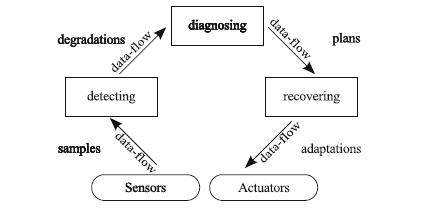
\includegraphics[width=5in]{img/Figure2}
\caption{The different stages of self-healing loops are:}
\end{figure}

\textit{Detect:} This stage filters any suspicious status data got from tests and reports recognized degradation.\\

\textit{Diagnose:} This stage incorporates root cause analysis, and computes a proper recuperation arrangement with the assistance of a policy base. (Self-healing policies)\\

\textit{Recovery:} This stage deliberately applies the arranged adjustments meeting the imperatives of the framework abilities and maintains a strategic distance from any unpredictable side effects.\cite{Harald:SelfHealingSurvey:2011}.   

\textbf{Version Two (Self-Healing Loop):\\}\\

\begin{figure}[H]
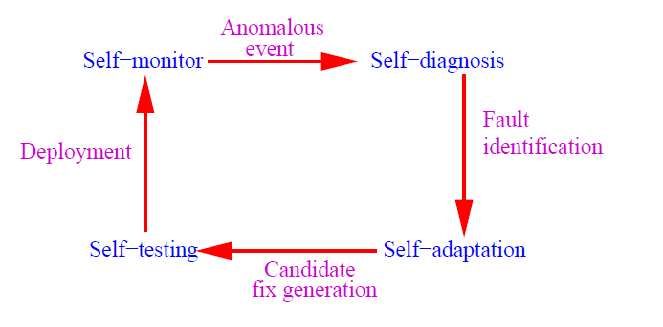
\includegraphics[width=5in]{img/Figure4}
\caption{The different stages of self-healing loops are:}
\end{figure}

The general architecture of a self-healing system can be divided in to four states: \\

\textit{1. Self-monitor:} In this state the system monitors for any abnormal or expected behaviour (Anomalous Event)\\

\textit{2. Self-diagnosis:} If such behaviours are detected, the system enters the self-diagnosis mode, where the main task is to fetch as much as information with respect to the specific fault that has been detected. The main goal of this identification stage is to detect the type of fault, the input/events which led the fault, the exact region in the code where the fault occurred and useful strategies for fixing the fault. (Fault Identification).\\

\textit{3. Self-adaption:} After identification the system needs to create one or more possible fixes with respect to the particular fault. Some of the important strategies to fix software faults include snapshot-rollback, input filtering, increased monitoring, isolation for the vulnerable process and selective application of any runtime protection mechanism.\\

\textit{4. Self-testing:} Depending on the efficiency of anyone of the fault-identification techniques. (e.g., in terms of side effects or performance degradation), we choose one of them. If an appropriate fix is produced the system is upgraded to the normalcy accordingly. The most important mechanisms for this are established patch-management and configuration-management. After figuring the best possible solutions.
\cite{Keromytis:SelfHealingSurvey:2011}.\\

\textbf{Version Three (Self-Healing Loop):\\}

The third version of the Self-Healing Loop defined by Ghosh et al. consists of three steps:   a) maintenance of the system health, (b) detection of system failure and (c) system recovery process. The Self-Healing Loop Is defined in the figure:

\begin{figure}[H]
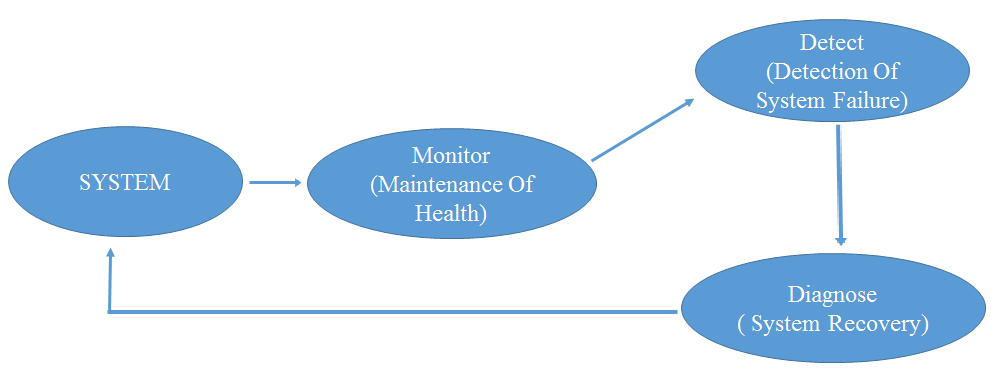
\includegraphics[width=5in]{img/pic1}
\caption{Steps Taken By A Self-Healing System When A Fault Occurs:}
\end{figure}

\textit{System Maintenance Of Health}
The system should check for faults periodically to
continue monitoring its health.There are various strategies that have been used to maintain the system health are:
1. Maintaining Redundancy
2. Maintenance By Probing
3. System Monitoring Model
4. Maintaining Diversity
5. Performance Log Analysis\\

\textit{Detection Of Failure}
Failure detection is another major area of research.Several approaches have been adopted
to detect non-self or abnormality in the functioning of the system are:
1. Missing Component/Message Response
2. System Monitoring Model
3. Foreign Element\\

\textit{System Recovery}
System recovery involves mechanisms to transform a system from an unhealthy state to a healthy state. 
This various redundancy techniques are:

1. Redundancy Techniques
2. Architectural Models And Repair Plans
3. Byzantine Agreement And Voting
4. Other Non-Traditional Methods
\cite{Ghosh:SelfHealingSurvey:2007}.\\

\chapter{Self-Healing Classification Schema} \label{ch:SelfHealingClassificationSchema}



\textbf{3.1. Domain:\\}
The surveyed literature has been classified by discussing the self-healing techniques that has been designed and implemented in the several applications areas. The different approaches are summarized in table 1.In each of the cases the table describes the self-healing approach and the techniques that has been used in each of the stages of the self-healing loops for detecting, diagnosing and recovering.
\cite{Harald:SelfHealingSurvey:2011}.\\

\begin{center}
    \begin{tabular}{ | p{3cm} | p{11cm} |}
    \hline
    Research Area & Summary \\ \hline
    Embedded Systems & Embedded systems are computer systems that are part of larger
systems and performs some of the requirements of these systems. Examples of such systems are auto mobile control systems, industrial processes control systems, mobile phones, or small sensor controllers. 
New ideas begin self-healing approaches to define recovery techniques focusing on the whole system instead of focusing on the recovery of individual components.
\cite{Harald:SelfHealingSurvey:2011}.
\cite{Crnkovic:SelfHealingSurvey:2005}.\\

\\ \hline
    Operating Systems & An operating system (OS) is a collection of software that allows a user or programmer to make use of the underlying hardware easier.New ideas begin a self-healing manager which keeps a track of the failures and re-runs the stopped services.
    
 \\ \hline
    Architecture Based & An Architecture- Based System is a conceptual model that defines the structure of a system. A system architecture is described using Architecture Description Languages (ADLs).New ideas begin with the help of architectural models expressed by architectural description language (ADL) differences between runtime composition and healthy model of composition are identified. \\
    \hline
    Cross/Multi-Layer-Base & A multi-layered software architecture is a software architecture that uses many layers for allocating the different responsibilities of a software product. New ideas begin with organizing the resources into layers. One approach uses the layers to avoid conflicts in resource allocation and other resource boundary and priorities.  \\ \hline
        Multi Agent-based & Multi-agent systems are distributed computing systems, that are composed of a number of interacting computational entities.New ideas begin in Agent-based environments act autonomously and host self-healing capabilities that protects the system part. 
 \\ \hline
     Reflective-middle-ware & New ideas begin on self-healing techniques on the middleware. This approach combines the properties of reflective middleware to self-healing enhancement.
 \\ \hline
      Legacy application and AOP & New ideas begin on self-healing techniques. The idea begins with finding checkpoints for monitoring recovery actions. This feature is provided by linker, runtime for legacy applications or implemented by aspect-oriented programming.
 \\ \hline
  Discovery systems and AOP & A discovery system is an artificial intelligence system which attempts to discover new scientific concepts or laws.
They are designed to support the discovery of different resources distinct requirements specified by individual semantics. New ideas begin that instead of deploying recovery strategy, try to keep request latency minimum and query responses consistent.
  \\ \hline
   Web services and QoS-based and AOP & New ideas begin with combining the monitoring and recovery capabilities to a self-healing loop. 
    \end{tabular}
\end{center}





\textbf{3.2. Technical Approach:\\}

Novel research ideas on Self-Healing Techniques\\

Some of the recent emergence of novel research ideas which addresses the issue of recovery in the presence of faults more efficiently are as follows. Amongst the below mentioned techniques: Failure-Oblivious Computing and Error Virtualization are termed as continued execution and are more highly valued than absolute correctness techniques (The method mentioned above)
\cite{Keromytis:SelfHealingSurvey:2011}.\\

\textit{3.2.1.Failure-Oblivious Computing:}
Failure oblivious computing mainly handles memory errors. In this technique the program code is extensively written to check for every memory access.
Failure-oblivious computing is a strategy that empowers computer programs to keep executing in spite of memory errors. The procedure handles endeavours to read invalid memory by returning back a manufactured value to the program. Thus in this strategy, no endeavour is made to advise the system that an error has occurred\\

\textit{3.2.2.Data-Structure Repair: }
This technique helps in detecting the corrupted data structures and fix it to a match with some pre-defined definitions/factors (Repair Algorithms). The Repair Algorithm produces a Data structure that satisfies consistency properties and is heuristically close to the broken data structure. In most cases it might not be necessary that the same data structure will be produced every time, but the new data structure must have some consistent property and keep the program operating successfully. The most common errors encountered in a Broken Data Structure Are Missing Elements, Inappropriate sharing, Dangling references, Out of bounds array indices and inconsistence values.\\
 
\textit{3.2.3.Error Virtualization: }
The main assumption in error virtualization is that a mapping can be made between the arrangement of set of errors that could happen at the time of program's execution and the restricted arrangement of errors that are explicitly taken care of by the project code.\\ 

By virtualizing the errors, an application can proceed with execution through a fault by invalidating the impacts of such faults and utilizing a manufactured return value for the function where the fault occurred. These return values were dictated by utilizing straightforward heuristics on the return type as controlled by source code analysis.\\

\textit{Smart Error Virtualization (SEV),} is another technique for self-healing that involves learning appropriate function return values at runtime.\\

\textit{3.2.4.Automatic Software Self-Healing Using Error Virtualization Rescue Points (ASSURE)}
ASSURE is an attempt to minize the probability of semantically incorrect response to a fault or attack. ASSURE technique proposes the concept of rescue points. Rescue points induce faults at areas that are known to propagate faults effectively, rather than attempting to mask errors to some previous technologies. The location in the code that handles these sort of anticipated faults leads to safe execution flow. This technique is very similar to exceptional handling that dynamically handles he best scoop to handle an error.\\

\textit{3.2.5.DIRA DIRA:}
DIRA is a technique for automatic detection, identification and repair of control-hijacking attacks. The technique is implemented as a GCC compiler. And uses checkpoints for detecting data structures when they are overwritten.\\

\textit{3.2.6.Vigilante Vigilante:}
This technique helps to detect vulnerability by executing injected code and defines a data-structure to handle this issue. The best part of this technique is that, it is exploit-argostic and is used against polymorphic worms.\\

\textbf{3.3. Steps:\\}

The diagram below shows the different Steps Involved In Survey Of Research In Self-Healing Systems:

\begin{figure}[H]
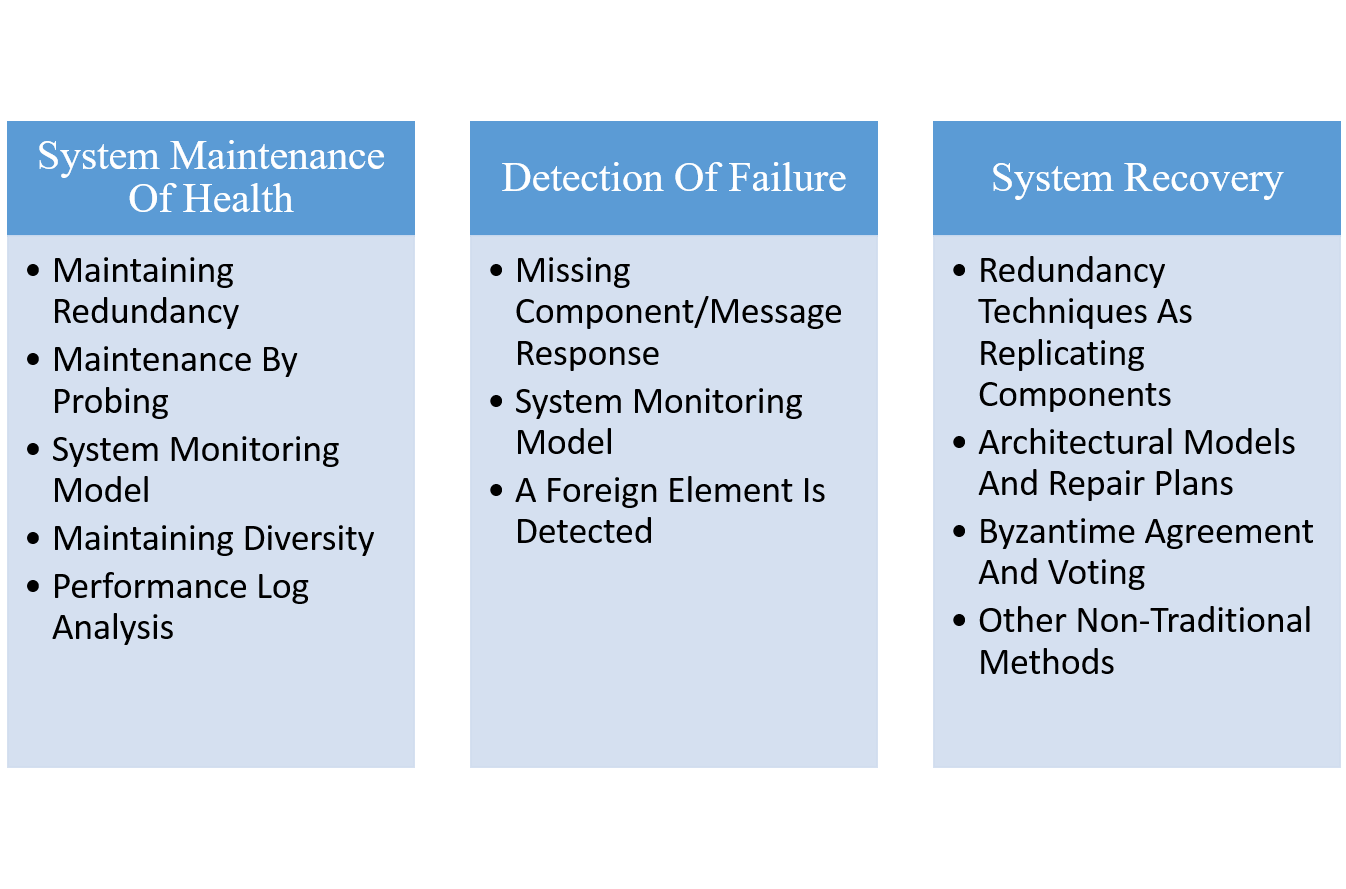
\includegraphics[width=5in]{img/SurveyofSelfHeaingResearch}
\caption{Survey Of Research In Self-Healing Systems:}
\end{figure}



\textbf{\textit{3.3.1.System Maintenance Of Health:}}
System Maintenance Of Health is a mechanism where the system should check for faults periodically to continue monitoring its health.There are various techniques that have been used to maintain the system health are:\\

\textit{1. Maintaining Redundancy:}
Replicating components to maintain redundancy is
always a popular choice in maintaining system health.There are many different redundancy strategies
that researchers in the area of self-healing have pursued.The most promising strategies discussed in this paper are\textit{:Cell Division, Self-Assembly and Multi-Agent Decision Making.}\\

\textit{2. Maintenance By Probing:}
Probing is a mechanism that is commonly used to get
information from the system in order to monitor its health.The different system probing procedures mentioned in the paper are: Grid Adaption/Coordinating SM,Decision And Control Layer,Feedback Control Loop,Adaptive Mirroring, Sensors Gathering Data From Functional Layer.\\

\textit{3. System Monitoring Model:}
Research in the area of self-healing systems includes
literature dealing with architecture models. The literature in this area has been broadly classified into three different categories:
(a) representing the system using Architectural Description Language (ADL), 
(b) representing regularities in a system, 
(c) providing a relational model of the system.\\

\textit{4. Maintaining Diversity:}
Diversity is an important strategy to attain system robustness. The different strategies using system diversity for maintaining system health are: Functionality Based Security, Diverse Design Model, Identify Critical Paths.\\

\textit{5. Performance Log Analysis:}\\
Performance log analysis is a scheme for the analysis of data on performance measures of the system, which can be used for the diagnosis of faults, the detection of intrusion and the facilitation of the healing process. The different strategies using performance log analysis for maintaining system health are: Watchtower, Predict Target Event, Finite Automata Scheme.\\

\textbf{\textit{3.3.2.Detection Of Failure:}}
Failure detection is another major area of research.Several approaches have been adopted
to detect non-self or abnormality in the functioning of the system are:\\

\textit{1. Missing Component/Message Response:}
This subsection discusses the policies where the strategy is to identify something missing from the normal behaviour of the system. Nagpal et al. propose a strategy in which the agents can produce replications when they sense the disappearance of their neighbours. The different strategies, for detecting failure  by sensing something a miss from the regular behaviour of the system are: Disappearance Of Components, Absence Of Message, Missing Response In Query.\\

\textit{2. System Monitoring Model:}
This subsection handles the policies which are suitable for architectures , where the system monitors components by probing.Merideth et al. propose a model in which pro-actively probing a system and collecting a data when a fault is detected improves the survivability of it. The different models for monitoring the system and detecting any failure are Monitoring Data For Trigger,Difference Between Running And Actual System, Parallel Space Servicing, Proactive Probing and Component Addition/Missing\\

\textit{3. A Foreign Element Is Detected:\\}
A proactive containment strategy notifies to the system the presence of a malicious replica.\\

\textbf{\textit{3.3.3.System Recovery:}}
System recovery involves mechanisms to transform a system from an unhealthy state to a healthy state. 
This various redundancy techniques are:\\

\textit{1. Redundancy Techniques As Replicating Components:}

Redundancy is the concept by which system can replicate components to replace dead neighbours and thus can recreate the entire structure.
Regeneration helps in recovering large part of effected system as long as the system has a circle center and enough reference points.The Redundancy techniques for healing are Self-Assembly Of Components, Replicating Cells and Recovery Oriented Computing Research.\\

\textit{2. Architectural Models And Repair Plans:}

In some cases, the Faulty components 
are isolated and the system is reconfigured 
with by incorporating different Repair Plans For Healing. The most important Plans For Healing are Use Of Gauges, Feedback Control Loops, Service and Contract (S+C) Protocol And Event Based Configuration.\\

\textit{3. Byzantine Agreement And Voting:}

For some systems, where the function of the system is to produce output results and the non-faulty components always produce the same value for the output, voting could take place and majority is applied to the output results of all process. In that way, faulty process can be detected and tolerated. (Merideth et al.). Another strategy is to delegate several agents to do the same task, and either select directly or vote on the agent that achieves the best complexity (on time, space, etc.) (Huhns et al).\\

\textit{4. Other Non-Traditional Methods}

Some Of the other non-traditional approaches used for system recovery are The Recovery-Oriented Computing Research Used at UC Berkley/Stanford and Failure Reporting Methodologies Used By The PSTN (public switched telephone network). 

\cite{Ghosh:SelfHealingSurvey:2007}.\\










%!TEX root =  main.tex
\appendix
\chapter{Detailed List of Self-Healing Approaches}
\label{ap:approches}

This appendix reports \ldots 

\section{} \label{}
\begin{compactitem}
\item[\textbf{Title}]Self-Adapting Reliability in Distributed Software Systems
\item[\textbf{Author}] 
Brun et al.
\item[\textbf{Reference}] 
\cite{brun_self-adapting_2015}
\item[\textbf{Year}] 
August, 2015
\item[\textbf{Application Domain}] 
Distributed computation architecture
\item[\textbf{Self-Healing steps}] Self-healing steps involved are fault-detecting, diagnosis and recovering
\item[\textbf{Technical Approach}]Iterative redundancy technique
\item[\textbf{Basic Idea}] 

The iterative redundancy algorithm is used to calculate the minimum of jobs to get a consensus, assuming that all the jobs produce the same result. The minimum number of jobs $d$ is calculated taking into account the system reliability $\mathbb{R}$ and node reliability $r$. The system reliability is used as a confidence threshold.

The minimum number of jobs $d$ is calculated taking into account the system reliability $\mathbb{R}$ and node reliability $r$, using the formulae:


 
$$\frac{r^d}{(1-r)^d+r^d}\geq \mathbb{R}$$




\item[\textbf{Summary of approach}]


Distributed computing architectures ensure the correct execution of each task through voting: multiple independent computational nodes perform the same task and if the majority of executions agree on a result, a consensus exists, and that result is taken to be the solution of that task. Iterative redundancy tries to optimize the use of computational nodes by distributing the minimum number of jobs that perform the same task required to achieve a desired confidence level in the result, assuming that all the jobs’ results agree. Then, if all jobs agree, the task is completed. However, if some results disagree, the confidence level associated with the majority result is diminished because of the chance that the disagreeing results are correct. The proposed approach then reevaluates the situation and distributes the minimum number of additional jobs that would achieve the desired level of confidence.
This process repeats until the agreeing results sufficiently outnumber the disagreeing results to reach the confidence threshold.


The flow-digram of the iterative redundancy algorithm is given by:
\begin{figure}[H]
\center
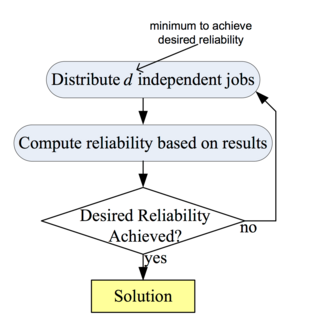
\includegraphics[width=5in]{img/Iterativeredundancyschematic}
\caption{Iterative redundancy schematic:}
\end{figure} 

\item[\textbf{Fault Types}]Byzantine attacks: A Byzantine fault is one where the faulty unit continues to run but produces incorrect results and might lead to failure sometimes. 

\item[\textbf{Failure Types}]Byzantine attacks.

\item[\textbf{Input data}] n independent jobs that perform the same jobs.

\item[\textbf{Recovery actions}]The technique try the deploy the redundant number of jobs in order to achieve consensus level.

\item[\textbf{Advantages}] Iterative redundancy is more cost effective as it creates the same level of software system reliability at a lower expense.

\item[\textbf{Disadvantages}] In iterative redundancy, the task server deploys several jobs and wait for the responses before possibly choosing to deploy more jobs. Therefore, this technique increases the latency for a particular task.

\item[\textbf{Case studies}]
The technique is implemented and tested on PlanetLab. PlanetLab is a gathering of PCs accessible as a testbed for distributed systems research.\\
\end{compactitem}


\begin{compactitem}
\item[\textbf{Title}]A Self-Healing Framework for Web-Based Applications (Showa)

\item[\textbf{Author}]Magalhães and Silva 

\item[\textbf{Reference}]

\cite{magalhaes_showa:_2015}

\item[\textbf{Year}] 2015

\item[\textbf{Application Domain}]
Web-based applications 

\item[\textbf{Self-Healing steps}] 
The self-healing steps involved are:Monitor, Plan, Analyze and Execute.

\item[\textbf{Technical Approach}]Data feeding and multiple statistical  analysis at various stages.

\item[\textbf{Basic Idea}] 
Various step by step modules have been used aiming to provide web-based applications the ability to detect performance anomalies during runtime and trigger automatic recovery actions to mitigate their impact. The framework (showa) gets loaded along with the web-based application during the start up, intercepts the running application to collect different system based and application based data. The collected data now gets prepared for two types of analysis:-workload variation analysis and performance anomaly analysis. Based on the outcome of these two analysis, the recovery planner module gets initiated and a specific recovery procedure is selected to be applied on the web application.

\item[\textbf{Summary of approaches}] 

The framework showa ensures the correct self healing recovery procedure through four processes:- monitor, plan, analyse and execute. Step by step modules consists of various statistical analysis, which are performed during the web application runtime to distinguish performance anomalies from workload variations, to detect the fault and approaching towards recovery procedure. The entire process consists of the following modules (1.sensor module, 2. data preparation module, 3.1. workload variation analysis module, 3.2.performance anomaly analysis module, 3.2.1.anomaly detector module, 3.2.2.root-cause failure analysis module, 4.recovery planner, 5.executor module and 6. effector module)

\begin{figure}[H]
\center
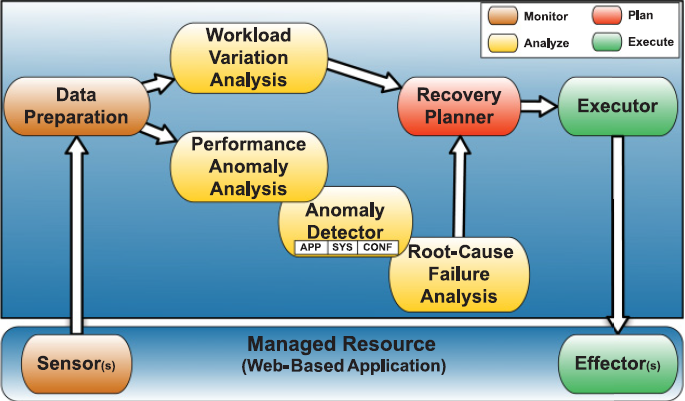
\includegraphics[width=5in]{img/selfhealingframework}
\caption{showa: self healing framework}
\end{figure}  

The sensor module monitors the system level performance and checks the status of the system services and performance ((CPU load, JVM heap memory, number of open files and number of running threads).). Additionally, it gathers execution time of application transactions without touching the source code. The data collected by the sensor module is passed on to the data preparation module. Here the time interval is determined of the collected data and the mix of transactions processed in an interval is characterized or identified. The prepared data is passed on to the next level of modules to detect and pinpoint if any anomaly is present. The data analysis is based on Spearman's rank correlation coefficient represented by rho(p). The correlation coefficient is given by the equation below and it expresses how two variables (X and Y) are associated.

\begin{figure}[H]
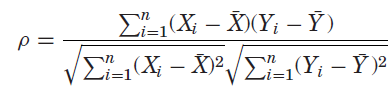
\includegraphics[width=5in]{img/formulae}
\caption{Measure of statistical dependence between two variables.}
\end{figure} 

where X is the sequence of the accumulated response server time per user transaction and Y is the number of user transactions processed in the same interval.If p remains stable and high across the periods of analysis, then it means that the response time is associated with the application workload. If p  decreases, then it means that one of the variables has increased or decreased while the other has remained stable or changed in an opposite direction. Considering the typical properties of modern distributed applications, this dissociation corresponds to a symptom of performance anomaly.

Anomaly detecting (Page:14). Performance Anomaly.

\item[\textbf{Fault types}]Fail-stutter fault. 

In fail-stutter faults, the components of a system sometimes fail and sometimes perform erratically (e.g., low performance) but are not reflected in the final results. These unexpected behaviors are defined as performance faults.

\item[\textbf{Failures types}]Fail-stutter fault

\item[\textbf{Input data}] The input are the parameters which are collected by the sensor module. For instance user transactions, CPU time per user transactions, amount of available memory.

\item[\textbf{Recovery actions}]The output are the recovery strategies which are carried forward or executed against the particular anomalies detected.

\item[\textbf{Advantages}] In showa sensor module the monitoring code is separated from the application code, thereby an application can be monitored without the need for manually changing its source code. With this separation, multiple applications can be monitored using the same monitoring code. The framework is generic and can be applied to any type of transactional web application. The only module that needs to be ported is the Sensor module

\item[\textbf{Disadvantages}]The ability to detect anomalies while the number of end users affected is low.

\item[\textbf{Case studies}]One retail store web application and an auction web application has been used in this paper for testing the framework.
\end{compactitem}



\begin{compactitem}
\item[\textbf{Title}]GenProg: A Generic Method for Automatic Software Repair

\item[\textbf{Author}]
Goues et al.   
\item[\textbf{Reference}]  

\cite{le_goues_genprog:_2012}

\item[\textbf{Application Domain}]
Real, unannotated programs with publicly documented bugs

\item[\textbf{Self-Healing steps:}]. The closed loop repair system works in this way. The method adopts an IDS (intrusion-detection system) that detects the anomalies in the system.

Whenever, the Intrusion Detection System,IDS detects an annomaly, GenProg is invoked to repair the suspicious behavior.

\item [\textbf{Technical Approach}] The method adopts an IDS (intrusion-detection system) that detects the anomalies in the system.

\item[\textbf{Basic Idea}] The program implements three functions:

The \textit{initialpopulation} generates the variants by using the mutual operators based on the input program and test cases.

The \textit{fitness function} evaluates each variants created and chooses the best amongst them.

The \textit{GenProg} iterates by selecting high fitness individuals, which are selected for continuous evolutions for the next.

\item[\textbf{Summary of approach}]
The technical approach used in this paper by the author can be classified in four stages:-
\textit{Program Representation:}Each variant is represented by a pair of an abstract syntax tree   (AST)and a weighted path. The abstract syntax tree contains all the statements of the program and a weighted path contains all the statements in the program that has been assigned a weight based on the occurrence of the statement the test cases.\\

\textit{Selection and Genetic Operators:}GenProg discards individuals with fitness 0 (variants that do not compile or that pass no test cases) and places the remainder in Viable. It then uses a selection strategy to select pop size/2 members of a new generation from the previous iteration.\\ 

\textit{Fitness function:}The fitness function evaluates the acceptability of a program variant. The fitness function mentioned in this paper, encodes software requirements at the test case level: negative test cases encode the fault to be repaired, while positive test cases encode functionality that cannot be sacrificed.\\

\textit{Repair Minimization:}

The search terminates successfully when GP discovers a primary repair that passes all test cases. Due to randomness in the mutation and crossover algorithms, the primary repair typically contains at least an order-of-magnitude more changes than are necessary to repair the program, rendering the repairs difficult to inspect for correctness.


\item[\textbf{Fault Types}]Infinite loop, Segmentation fault, Remote heap buffer over flow to inject code, Remote heap buffer overflow to overwrite variables, Non overflow denial of service, Local stack buffer overflow, Integer overflow and Format string vulnerability.

\item[\textbf{Input data}] Input source code contains a failing negative test case that exercises the defect and a set of passing positive test cases that describe requirements.

\item[\textbf{Recovery actions}]The recovery action is the primary repair that passes all test cases.

\item[\textbf{Advantages}] 
The GP search space focuses genetic operations along a weighted path and takes advantage of test case coverage information, and reusing existing program statements.

\item[\textbf{Disadvantages}] GenProg relies on test cases to encode both an error to repair and important functionality. GenProg cannot repair race conditions as it is difficult to encode an error using test cases for non-deterministic properties.


\end{compactitem}



\begin{compactitem}

\item[\textbf{Title}]Exception Handling for Repair in Service-Based Processes

\item[\textbf{Author}]Friedrich et al.

\item[\textbf{Reference}] 

\cite{friedrich2010exception}

\item[\textbf{Year}] 2010

\item[\textbf{Application Domain}]
Service-based processes

\item[\textbf{Self-Healing steps}] The self healing loop is: design, diagnosis, repair


Diagnosis: This phase determines where the error took place and what the cause of the error is. The knowledge about the fault is crucial for repairing the process and for minimizing the need for re executing parts of the process. Such knowledge is obtained through diagnosis,  using a diagnosis tool.

\item[\textbf{Technical Approach}]Model based approach

\item[\textbf{Basic Idea}] In this paper, we design repair strategies based on the structure of the process by using model-based approach. The repair plan / actions is defined in the process model. The approach is based on the concept of self-healing system. In this approach, the repair information is associated with a process at design time and the repair plans are generated at runtime.

\item[\textbf{Summary of approach}]

\item[\textbf{Fault Types}]The two types of faults that can be healed in this case are: 

\item[\textbf{Failure Types}]The two types of faults that has been healed in this case are:

An incorrect item code with an item name. The system send a wrong shipping note to warehouse, which therefore does not process the order and the package correctly.


When the are house receives the item description from the SHOP through the FORWARDORDER operation, it discovers that the order goods, the shipping note and the package are inconsistent with respect to the goals provided by the supplier and thus raised failure 1.

\item[\textbf{Input data}] 

\item[\textbf{Recovery actions}]

\item[\textbf{Advantages}] 
Repair follows the same logic as the original process and different repairs can be proposed for different causes of failures, with the goal of minimizing both the amount of work to be redone in the process and the compensation and/or reexecution of external services.

\item[\textbf{Disadvantages}] 



\item[\textbf{Case study}] 


The approach has been used on a food shop selling company, which sells products online using a service-oriented architecture (SDA) infrastructure with four services.

\end{compactitem}











\bibliographystyle{plain}
\bibliography{biblio}
\end{document}
